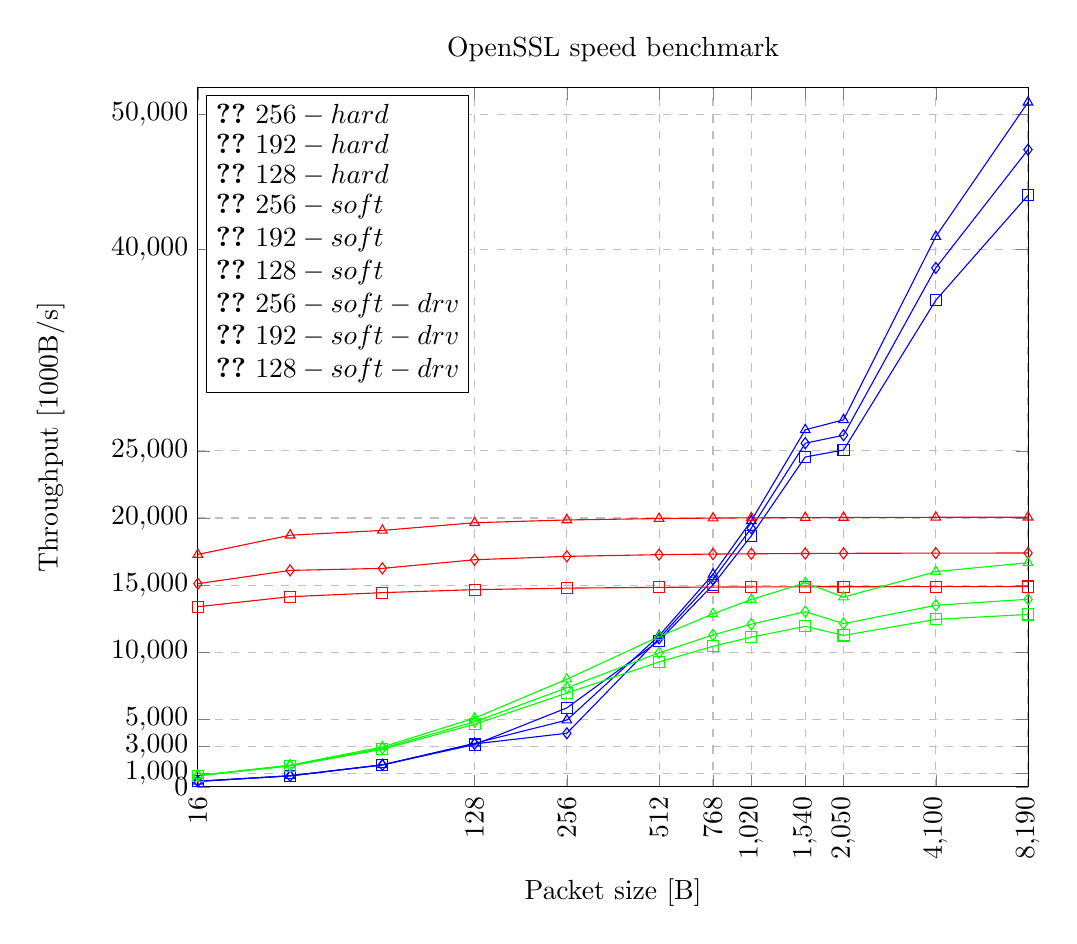
\begin{tikzpicture}
\begin{semilogxaxis}[
	width=\linewidth,
    title={OpenSSL speed benchmark},
    xlabel={Packet size [B]},
    ylabel={Throughput [1000B/s]},
    ylabel shift = 1 em,
    xmin=16, xmax=8200,
    ymin=0, ymax=52000,
    xtick={16,128,256,512,768,1024,1536,2048,4096,8192},
    x tick label style={rotate=90,anchor=east,/pgf/number format/fixed},
    log ticks with fixed point,
    ytick={0,1000,3000,5000,10000,15000,20000,25000,40000,50000},
    legend pos=north west,
    xmajorgrids=true,
    ymajorgrids=true,
    grid style=dashed,
    scaled ticks=false,
    y tick label style={/pgf/number format/fixed},
    log basis x={2},
]

% For all these tests:
% OpenSSL 1.0.1j 15 Oct 2014
% built on: Tue Apr 21 13:19:30 CEST 2015
% options:bn(64,32) rc4(ptr,char) des(idx,cisc,16,long) aes(partial) idea(int) blowfish(ptr)
% compiler: arm-linux-gnueabihf-gcc -fPIC -DOPENSSL_PIC -DOPENSSL_THREADS -D_REENTRANT -DDSO_DLFCN -DHAVE_DLFCN_H -fPIC -DHAVE_CRYPTODEV -DUSE_CRYPTODEV_DIGESTS -I/PROJECTS/CryptoSoC/qude/toolchain/cryptodev-linux-master -fno-omit-frame-pointer -fno-inline -g -marm -DTERMIO -O3 -Wall
% Configured with ./Configure linux-armv4 shared -fPIC --openssldir=/usr/local --cross-compile-prefix="arm-linux-gnueabihf-" --install_prefix=/PROJECTS/CryptoSoC/qude/toolchain/openssl_compiled_noasm_fp_cryptodev_patch_condoff -DHAVE_CRYPTODEV -DUSE_CRYPTODEV_DIGESTS -I/PROJECTS/CryptoSoC/qude/toolchain/cryptodev-linux-master -fno-omit-frame-pointer no-asm -fno-inline -g -marm
% When hard: ba411e built 2015-02-24, IRQ, no dbg
 
\addplot[
    color=blue,
    mark=square,
    ]
    coordinates {
    (16,404.67)(32,820.25)(64,1633.24)(128,3145.30)(256,5871.70)(512,10867.20)(768,15028.74)(1024,18676.74)(1536,24540.16)(2048,25055.23)(4096,36197.72)(8192,44007.42)
    };
    \label{aes-256-cbc-hard}
 
\addplot[
    color=blue,
    mark=diamond,
    ]
    coordinates {
    (16,411.34)(32,818.45)(64,1630.19)(128,3195.09)(256,3984.81)(512,11039.57)(768,15429.38)(1024,19244.71)(1536,25562.62)(2048,26161.15)(4096,38600.70)(8192,47401.64)
    };
    \label{aes-192-cbc-hard}
 
\addplot[
    color=blue,
    mark=triangle,
    ]
    coordinates {
    (16,411.65)(32,820.29)(64,1633.00)(128,3238.91)(256,4964.95)(512,11240.28)(768,15811.33)(1024,19797.67)(1536,26562.56)(2048,27302.57)(4096,40936.79)(8192,50929.66)
    };
    \label{aes-128-cbc-hard}
 
\addplot[
    color=red,
    mark=square,
    ]
    coordinates {
    (16,13400.87)(32,14146.01)(64,14446.53)(128,14669.01)(256,14783.06)(512,14840.83)(768,14860.29)(1024,14870.19)(1536,14879.74)(2048,14885.55)(4096,14893.06)(8192,14898.52)
    };
    \label{aes-256-cbc-soft}
 
\addplot[
    color=red,
    mark=diamond,
    ]
    coordinates {
    (16,15115.54)(32,16101.85)(64,16251.20)(128,16894.55)(256,17145.26)(512,17272.66)(768,17315.84)(1024,17337.34)(1536,17359.36)(2048,17371.14)(4096,17387.52)(8192,17394.35)
    };
    \label{aes-192-cbc-soft}
 
\addplot[
    color=red,
    mark=triangle,
    ]
    coordinates {
    (16,17289.54)(32,18720.89)(64,19076.29)(128,19649.24)(256,19854.42)(512,19958.78)(768,19993.86)(1024,20011.35)(1536,20028.93)(2048,20039.00)(4096,20052.65)(8192,20059.48)
    };
    \label{aes-128-cbc-soft}
 
\addplot[
    color=green,
    mark=square,
    ]
    coordinates {
    (16,825.74)(32,1552.37)(64,2792.81)(128,4654.46)(256,6975.40)(512,9292.63)(768,10454.53)(1024,11138.39)(1536,11941.38)(2048,11264.68)(4096,12460.03)(8192,12825.94)
    };
    \label{aes-256-cbc-soft-drv}
 
\addplot[
    color=green,
    mark=diamond,
    ]
    coordinates {
    (16,835.37)(32,1584.03)(64,2870.98)(128,4836.39)(256,7370.07)(512,9970.18)(768,11301.38)(1024,12102.66)(1536,13032.96)(2048,12142.59)(4096,13508.61)(8192,13953.71)
    };
    \label{aes-192-cbc-soft-drv}
 
\addplot[
    color=green,
    mark=triangle,
    ]
    coordinates {
    (16,844.73)(32,1614.79)(64,2967.79)(128,5114.41)(256,8011.09)(512,11178.67)(768,12875.52)(1024,13933.91)(1536,15181.82)(2048,14113.45)(4096,16012.63)(8192,16673.45)
    };
    \label{aes-128-cbc-soft-drv}

\node [draw,fill=white,anchor=north west] at (rel axis cs: 0.01,0.99) {\shortstack[l]{
        \ref{aes-256-cbc-hard} $256-hard$ \\
        \ref{aes-192-cbc-hard} $192-hard$ \\
        \ref{aes-128-cbc-hard} $128-hard$ \\
        \ref{aes-256-cbc-soft} $256-soft$ \\
        \ref{aes-192-cbc-soft} $192-soft$ \\
        \ref{aes-128-cbc-soft} $128-soft$ \\
        \ref{aes-256-cbc-soft-drv} $256-soft-drv$ \\
        \ref{aes-192-cbc-soft-drv} $192-soft-drv$ \\
        \ref{aes-128-cbc-soft-drv} $128-soft-drv$}};
 
\end{semilogxaxis}
\end{tikzpicture}